\chapter{(E) Processi stocastici} \label{cap:bimodal}

\section{(E-0) Sviluppo del processo lognormale a variabile stocastica binaria}

La determinazione del prezzo di un prodotto derivato è indissolubilmente legata all'andamento teorico del valore del sottostante. Data questa premessa, un equo \textit{pricing} di opzione non può prescindere da una previsione il più accurata possibile dell'andamento di tale valore. Nella Sezione introduttiva \ref{sec:introduction_econophysic_option_pricing} è stato indicato lo schema del \textit{moto browniano geometrico} come particolarmente valido per questo tipo di modellizzazione. Il processo lognormale con cui evolve il prezzo del sottostante è quindi un processo di tipo \textit{markoviano} descritto, come si è visto, dall'Equazione a \textit{schema esatto} \eqref{eq:exactprice}, dove $w$ rappresenta una variabile aleatoria a media nulla e varianza unitaria.

Nell'ottica di riprodurre con la maggiore fedeltà possibile un'ipotetica evoluzione dei prezzi del sottostante, tale termine è stato estratto da una distribuzione gaussiana. Successivamente, a titolo di confronto, abbiamo implementato una nuova funzione per applicare iterativamente il processo lognormale con una variabile stocastica dicotomica. La indichiamo con $z$:
\begin{equation}
    z = \begin{cases}
    +1, & \text{con probabilità} \,\, \frac{1}{2};\\
    -1, & \text{con probabilità} \,\, \frac{1}{2}.
  \end{cases}
    \label{eq:binary_variable}
\end{equation}
Consideriamo ora la legge di sviluppo del prezzo dell'opzione
\begin{equation}
    S(t_0 + \Delta t) = S(t_0) e^{(r - \frac{\sigma^2}{2}) \Delta t + \sigma \sqrt{\Delta t} z}
    \label{eq:bimodal_price}
\end{equation}
e l'effetto determinato dalla conversione di $w$ gaussiana in $z$ binaria.

Per ogni intervallo temporale $\Delta t$ il valore di $S(t_{i + 1})$ è vincolato a due sole possibilità rispetto a $S(t_i)$, ovvero quella di un movimento al rialzo, nel caso $z = 1$, o al ribasso, se $z = 0$. A ogni passo della simulazione il prezzo $S(t)$ può quindi assumere due soli valori dipendenti dal risultato del passo precedente, dalla volatilità $\sigma$, dal \textit{risk free rate} $r$ e dalla scelta dell'intervallo stesso $\Delta t$, in contrapposizione al continuo di valori del processo lognormale standard.

\section{(E-1) Convergenza del processo binario al processo lognormale gaussiano}

Sia che si scelga di utilizzare una variabile $w$ a distribuzione gaussiana, sia che il termine aleatorio sia di tipo bimodale $z$, la funzione \codeword{ExactLogNormalStep}, che prende in ingresso la variabile stocastica e restituisce il prezzo del sottostante alla data di rilevazione considerata, è la medesima, in quanto l'Equazione \eqref{eq:exactprice} si applica identicamente all'uno e all'altro caso. 

Attraverso uno script che cicla lungo una serie di file di testo con valori diversi del parametro di \textit{input} relativo alle date di rilevazione, abbiamo eseguito una serie di coppie di simulazioni identiche salvo il tipo di parametro pseudocasuale passato alle funzioni del processo lognormale. In questo modo è stato possibile confrontare i risultati relativi a entrambe le scelte di termine aleatorio per verificarne la convergenza.

In particolare, le simulazioni prese in esame per la comparazione stimano il prezzo a \textit{tempo di maturità} di un anno di opzioni del tipo \textit{Plain Vanilla Call}. I numeri di blocchi e di \textit{thread} per blocco sono rispettivamente $50$ e $512$, per un totale di $10000000$ di simulazioni. I dati di mercato, anch'essi fissi, stabiliscono il \textit{prezzo iniziale} a $100\$$, \textit{volatilità} pari a $0.25$ e \textit{tasso d'interesse privo di rischio} allo $0.01\%$. Il numero di intervalli temporali varia da $1$ a $350$. Schematizzati in Figura \ref{fig:bimodal} sono riportati i risultati ottenuti per mezzo del processo lognormale esatto.

\begin{figure}[t]
    \centering
    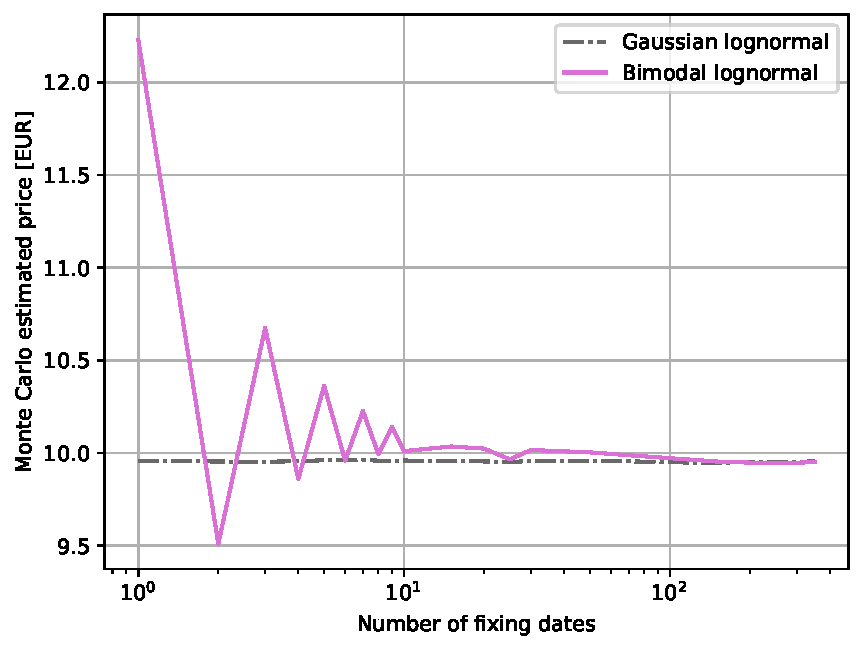
\includegraphics[scale=0.5]{graphs/OptionPriceBimodal_PriceVsM.pdf}
    \caption{Prezzo stimato dell'opzione \textit{performance corridor} tramite lo schema lognormale esatto sfruttando variabili pseudocasuali bimodali (\textit{rosso}) e gaussiane di media nulla e varianza unitaria (\textit{nero, tratteggiato}.}
    \label{fig:bimodal}
\end{figure}

L'evoluzione delle due curve incontra le nostre aspettative. Si nota infatti come, dopo un'iniziale fase discordante, i due sviluppi tendano a sovrapporsi e in particolare sia l'andamento della curva a variabile bimodale a stabilizzarsi fino a convergere sui risultati di quella a variabile gaussiana. La spiegazione risiede nella natura \textit{markoviana} del processo di calcolo: lo schema lognormale si basa su una successione ricorsiva che estrapola il prezzo al tempo $t_i$ a partire da quello alla data precedente $t_{i-1}$. Di conseguenza, nel caso non ci siano <<tappe temporali intermedie>>, i prezzi al \textit{tempo di maturità} sono l'esito di un'unica operazione in positivo o negativo. I risultati ottenuti dal singolo \textit{thread} si raggruppano dunque in due classi di prezzi, molto dispersi rispetto al <<valore limite>>. Incrementando il numero di passaggi intermedi aumenta il ventaglio di prezzi ottenibili dalla singola simulazione e i risultati vanno a occupare con maggiore probabilità le classi di prezzo più vicine al limite. Per una densità di date di rilevazione sufficientemente elevata i due processi danno risultati confrontabili, sebbene l'impiego di una variabile dicotomica non permetta di parlare di tendenza asintotica; infatti, al crescere di $m$ il prezzo finale del metodo binario non si avvicina <<dall'alto>> o <<dal basso>> al valore gaussiano, ma mantiene un carattere oscillante.

Quanto appena esposto è giustificato dal \textit{Teorema del limite centrale}, secondo il quale la somma e la media di variabili aleatorie indipendenti e con la medesima distribuzione, qualunque essa sia, tendono ad assumere una distribuzione gaussiana.

Considerando ora l'equazione che descrive l'andamento del prezzo del sottostante in relazione a $\Delta t$ e al numero $q$ di sottointervalli temporali di rilevazione
\begin{equation}
    S(n \Delta t) = S(t_0) e^{n (r - \frac{\sigma^2}{2}) \Delta t + \sigma \sqrt{\Delta t} \displaystyle\sum_{i=1}^q w_i}
    \label{eq:price(n)}
\end{equation}
si può pensare di ridefinire $\displaystyle\sum_{i=1}^q w_i$ come nuova variabile aleatoria $Y(q)$. Questo accorgimento è giustificato dal fatto che le ${w_i}$ sono termini pseudocasuali indipendenti e legati a una medesima distribuzione. Essendo soddisfatte le ipotesi del \textit{Teorema del limite centrale}, $Y(q)$ deve essere una variabile a distribuzione normale con varianza pari alla varianza delle ${w_i}$, cioè unitaria. Per $q$ sufficientemente alto quindi, anche nel caso della variabile bimodale la \eqref{eq:price(n)} si riconduce a un'equazione dipendente da un parametro gaussiano $Y(q)$. L'andamento osservato sperimentalmente ha quindi una comprova teorica.
